\documentclass{ctexart}
\usepackage[a4paper,top=2cm,bottom=2cm,left=3cm,right=3cm,marginparwidth=1.75cm]{geometry}

\usepackage{amsmath}
\usepackage{graphicx}
\usepackage[colorlinks=true, allcolors=blue]{hyperref}
\usepackage{CJKutf8}
\usepackage{CJKpunct}

\title{物质运输}
\author{笙}

\begin{document}
\tableofcontents
\maketitle


\begin{abstract}
生物.必修一.第四章.
\end{abstract}

\section{被动运输}

\subsection{渗透作用}

\subsubsection{概念}

扩散作用：物质从相对含量多的地方向少的地方自由运动。

渗透作用：水分子或溶剂分子通过\textbf{半透膜}进行扩散，需要半透膜\textbf{两侧具有浓度差}。

半透膜：物质能否通过膜取决于分子的大小。

选择透过性膜：物质能否通过取决于生物活细胞的选择性。

\begin{figure}[h]
\centering
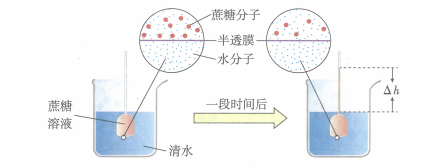
\includegraphics[width=0.8\linewidth]{Pic1.png}
\end{figure}

渗透方向的判断：

1.水相对含量高$\longrightarrow$水相对含量低。

2.低浓度溶液$\longrightarrow$高浓度溶液。

3.渗透压低$\longrightarrow$渗透压高。

\subsubsection{渗透平衡}

当蔗糖溶液与清水之间渗透压之差$=$高度差$\delta h$产生的压强，液面维持稳定。

\bigskip

Question:

1.渗透作用中水的运输方向是单向还是双向的吗？

2.渗透作用等于扩散作用吗？

\subsection{水进出细胞的原理}

\subsubsection{植物细胞的吸水和失水}

条件：\textbf{活的、成熟的、具有中央大液泡的}植物细胞。

原理：

\begin{figure}[h]
\centering
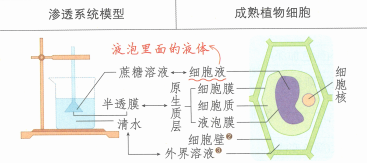
\includegraphics[width=0.8\linewidth]{Pic2.png}
\end{figure}

外界溶液浓度高时，植物细胞失水，发生\textbf{质壁分离}现象。

\textbf{植物细胞吸水不会破裂}，因为细胞壁起支持和保护的作用。

植物细胞壁和细胞膜之间是\textbf{外界溶液}，细胞壁具有\textbf{全透性}。

\subsubsection{动物细胞的吸水和失水}

原理：\textbf{细胞膜}相当于半透膜，细胞质与外界溶液间存在浓度差。

现象：

\begin{figure}[h]
\centering
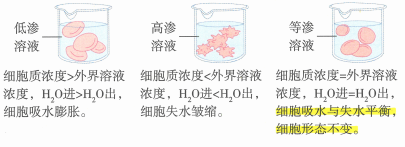
\includegraphics[width=0.8\linewidth]{Pic3.png}
\end{figure}

\subsection{实验：探究植物细胞的吸水和失水}

\subsubsection{原理}

1.内因：成熟的植物细胞的\textbf{原生质层}相当于一层半透膜；原生质层的伸缩性大于细胞壁。

2.外因：细胞液与外界溶液存在浓度差。

\subsubsection{步骤}

选材、制片：紫色洋葱鳞片叶外表皮(具有中央液泡，细胞液带有颜色)或叶肉细胞(原生质层为绿色，细胞液无色透明)。

观察：紫色的中央液泡，原生质层紧贴细胞壁。

滴高渗溶液：滴加质量浓度为$0.3g/mL$蔗糖溶液，用吸水纸引流。

观察：中央液泡变小，颜色加深；原生质层与细胞壁逐渐分离。

滴清水：吸水纸引流。

观察：中央液泡变大，颜色变浅；原生质层与细胞壁贴近。

\subsection{被动运输——自由扩散和协助扩散}

被动运输：物质以扩散的方法进出细胞，无需细胞消耗能量。

\subsubsection{分类}

\begin{table}[h]
    \centering
    \begin{tabular}{|c|c|c|}
        \hline
             & 自由扩散 & 协助扩散(易化扩散) \\
        \hline
        方向 & 顺浓度梯度 & 顺浓度梯度\\
        \hline
        转运蛋白 & 不需要 & 需要 \\
        \hline
        例子 & 甘油、乙醇、苯、性激素(脂溶性小分子) & 葡萄糖进入成熟红细胞\\
            & $O_2$和$CO_2$ & 水分子借助水通道蛋白进入细胞\\
        \hline
        影响因素 & 浓度差 & 浓度差；蛋白数量\\
        \hline     
    \end{tabular}
\end{table}

\subsubsection{转运蛋白的分类}

\begin{figure}[h]
\centering
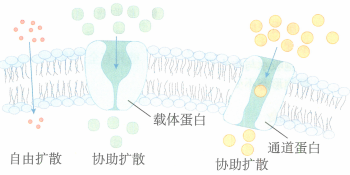
\includegraphics[width=0.8\linewidth]{Pic4.png}
\end{figure}

通道蛋白：允许与自身通道直径和形状适配、大小和电荷相适宜的分子通过；分子或离子通过通道蛋白时不需要与其结合。

载体蛋白：允许与自身结合部位相适应的分子或离子通过；每次转运均伴随自身构象的改变。

\section{主动运输与胞吞胞吐}

\subsection{主动运输}

主动运输：物质\textbf{逆浓度梯度}进行跨膜运输，需要载体蛋白协助，耗能。

\textbf{相同物质进入不同细胞的跨膜运输方式可能不同}。例如，人的成熟红细胞吸收葡萄糖的方式为协助扩散，而小肠上皮细胞吸收葡萄糖的方式为主动运输。

\subsection{胞吞和胞吐}

\begin{figure}[h]
\centering
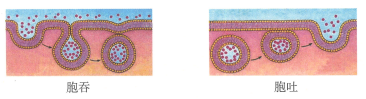
\includegraphics[width=0.6\linewidth]{Pic5.png}
\end{figure}

胞吞：大分子物质与细胞膜上的蛋白质结合后，细胞膜内陷分离形成囊泡，大分子物质随之进入细胞。

胞吐：大分子物质进入囊泡，囊泡与细胞膜融合排出细胞。

特点：耗能；借助膜的融合完成，与流动性相关；不需要转运蛋白，但需要膜上蛋白质的参与。


\end{document}